\chapter{Public Key Cryptography}
\label{chap:public}

We now talk about \gls{publiccrypto}.



\section{The Need for Public Key Cryptography}

Alice and Bob would like to communicate with each other.
Unfortunately, there is a problem:
they have never met and are not able to meet beforehand.
Thus, they are not able to share a secret through a \gls{secure channel}.
Is there some way that Alice and Bob can still securely communicate
over an \gls{insecure channel}?
The answer is yes, and communication is possible using
\emph{\gls{publiccrypto}}.

In each case, Alice and Bob have \emph{two} keys:
a \emph{public key} (known to everyone) and
a \emph{private key} (known only to the individual).
We recall that in \gls{symmetriccrypto},
Alice and Bob \emph{share} a secret key.
Due to the nature of the private key, it should never be shared;
see Figure~\ref{fig:xkcd_public_key}.

\begin{figure}[t]
\centering
    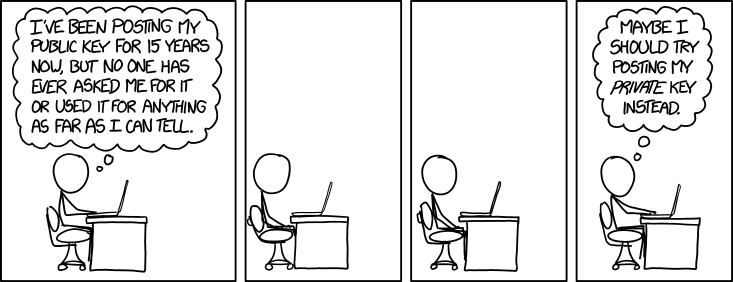
\includegraphics[width=0.75\textwidth]{figures/xkcd/xkcd_1553_public_key.png}
    \caption[\texttt{xkcd} Public Key]{Even with a lack of attention,
        posting one's private key is \emph{highly} discouraged.
        Created by Randall Munroe on \texttt{xkcd};
        posted online at \url{https://xkcd.com/1553/}.
        }
    \label{fig:xkcd_public_key}
\end{figure}


The \gls{dhke} was first described in
by Diffie and Hellman in~\cite{DHKEpaper}.
The first method for performing \gls{public key encryption}
and \glspl{signature} was the original RSA paper~\cite{RSApaper}
by Rivest, Shamir, and Adleman.
We will not discuss \gls{publiccrypto} based on RSA;
these notes focus on \gls{ecc}.



\section{Brief Discussion of Public Key Infrastructure}

\Gls{publiccrypto} \emph{assumes} the ability for Alice and Bob
to publicly post information and allow everyone to know
that this information is valid.
This is handled by Public Key Infrastructure (PKI).
This is an important aspect of \gls{publiccrypto}
and is also very challenging; we will not go into details at this time.
For simplicity, we will assume that such infrastructure is present.



\section{Diffie-Hellman Key Exchange}
\label{sec:public_diffie_hellman}

Here, we discuss how Alice and Bob, who have never met,
can construct a \gls{shared secret}.
This \gls{shared secret} may then be used derive a secret key
for \gls{symmetric key encryption}.

\subsection{Intuition and Discussion}

We would like to use mathematics to help Alice and Bob communicate.

Let $G$ be a \gls{cyclic group} with generator $g$ and order $\abs{G} = N$.
W let $a,b\chooseRandom{}\Z_{N}^{*}$ be private keys and $g^{a},g^{b}\in G$
be the corresponding public keys.
We want to be able to combine this information in some way to derive
a \gls{shared secret} that Alice and Bob can use to securely communicate
over an \gls{insecure channel}.
At the same time, it should be impractical for eavesdropper Eve
to derive the \gls{shared secret} from the public information.

If Alice has Bob's public key $g^{b}$, then she can compute

\begin{equation}
    \parens{g^{b}}^{a} = g^{ab}.
\end{equation}

\noindent
Similarly, if Bob has Alice's public key $g^{a}$, then he can compute

\begin{equation}
    \parens{g^{a}}^{b} = g^{ab}.
\end{equation}

\noindent
Thus, $g^{ab}$ is a secret that both Alice and Bob can compute.
This is their \emph{\gls{shared secret}}.

If it is difficult to compute $g^{ab}$ given $g^{a}$ and $g^{b}$,
then this method enables Alice and Bob to compute a \gls{shared secret}
which is hard for Eve to determine.
This \gls{shared secret} can then be used to derive a secret key
for secure communication using \gls{symmetric key encryption}.
\emph{Deriving} a key from the \gls{shared secret} and
not using the shared secret directly is important for security.
Some form of \emph{\gls{kdf}} (KDF) is generally used;
we briefly mentioned KDFs based on \glspl{hash function}
in Chapter~\ref{sec:hash_hkdf}.

\begin{example}[DH Example 1]
\exampleCodeReference{examples/public/diffie-hellman\_1.py}

We now go through an example.
Let us look at $\F_{7919}$; we let $7\in\F_{7919}$ be the base point.
It can be shown that $\angles{7} = \F_{7919}^{*}$
so that $\abs{\angles{7}} = 7918$;
for more information, see Appendix~\ref{app:math_finite_fields_primitive} and
Example~\ref{example:app_math_finite_generator_7919}.

We let $a = 3545$ and $b = 6614$.
Here, $a$ is Alice's private key and $b$ is Bob's private key.
In this case, we have

\begin{align}
    A &\mathDef{} 7^{3545} \mod 7919 \nonumber\\
        &= 5490 \nonumber\\
    B &\mathDef{} 7^{6614} \mod 7919 \nonumber\\
        &= 407,
\end{align}

\noindent
where $A$ is Alice's public key and $B$ is Bob's public key.

Now, Alice knows $B$ and computes $B^{a}$ to learn their \gls{shared secret}:

\begin{align}
    B^{a} &= 407^{3545} \mod 7919 \nonumber\\
        &= 4439.
\end{align}

\noindent
Similarly, Bob knows $A$ and computes $A^{b}$:

\begin{align}
    A^{b} &= 5490^{6614} \mod 7919 \nonumber\\
        &= 4439.
\end{align}

\noindent
They can now derive a secret key from their \gls{shared secret} $4439$.
\end{example}

\begin{example}[DH Example 2]
\exampleCodeReference{examples/public/diffie-hellman\_2.py}

We now go through another example.
The setup is the same:
we look at $\F_{7919}$ and let $7\in\F_{7919}$ be the base point.

We let $a = 1347$ and $b = 4862$.
Then

\begin{align}
    A &\mathDef{} 7^{1347} \mod 7919 \nonumber\\
        &= 683 \nonumber\\
    B &\mathDef{} 7^{4862} \mod 7919 \nonumber\\
        &= 2710.
\end{align}

Alice computes

\begin{align}
    B^{a} &= 2710^{1347} \mod 7919 \nonumber\\
        &= 7114.
\end{align}

\noindent
Bob computes

\begin{align}
    A^{b} &= 683^{4862} \mod 7919 \nonumber\\
        &= 7114.
\end{align}

\noindent
They can derive a secret key from their \gls{shared secret} $7114$.
\end{example}

\subsection{Formal Definition}

We now give the formal definition.
This definition holds for any \gls{cyclic group}.

\begin{defn}
\label{def:diffie-hellman}
Let $G = \angles{g}$ and $\abs{G} = N$.
Choose $a,b\chooseRandom{}\Z_{N}^{*}$ as private keys and set
$A = g^{a}$ and $B = g^{b}$.
Then $A,B\in G$ are public keys.

The \emph{\gls{shared secret}} is $g^{ab}\in G$.
We have

\begin{align}
    B^{a} &= \parens{g^{b}}^{a} \nonumber\\
        &= g^{ab}
\end{align}

\noindent
and

\begin{align}
    A^{b} &= \parens{g^{a}}^{b} \nonumber\\
        &= g^{ab}.
\end{align}
\end{defn}

\subsection{Potential Confusion between Public and Private Keys}

Care must be taken to avoid confusion between private keys
and public keys.
From the definition, the private key is a element of $\Z_{N}^{*}$
while the public key is an element of $G$;
that is, the private key is an \emph{integer}
and the public key is a \emph{group element}.

Potential confusion may arise from the fact that when we are
using \glspl{subgroup} of $\F_{p}$ (so that $G\le \F_{p}$),
then both the private key \emph{and} the public key are integers.
This may cause some initial confusion when trying to understand the
\gls{dhke}.
In Chapter~\ref{sec:ecdh}, we look at the \gls{dhke}
using \glspl{subgroup} of \glspl{elliptic curve}.
In that case, the private key is an integer while the public key
is a point on an \gls{elliptic curve}.

\subsection{Security of the \glsentrytext{dhke}}

A discussion of the security of the \gls{dhke} can be found
in Chapter~\ref{chap:hardness}.



\section{Elgamal Encryption}
\label{sec:public_elgamal_encryption}

We now describe the Elgamal \gls{encryption scheme}~\cite{elgamal1985public}.

The \gls{dhke} made it possible to compute a \gls{shared secret}
from two public keys;
that \gls{shared secret} is the used to derive a secret key
for \gls{symmetric key encryption}.
We now will consider the situation where encryption is based
on the public key.

\subsection{Formal Definition}

\begin{defn}
We let $G$ be a \gls{cyclic group} with generator $g$ of order $N$.

\paragraph{Key Generation}
Let $x\chooseRandom{}\Z_{N}^{*}$ be the private key.
The public key is $g^{x}$.

\paragraph{Encryption}
Alice wishes to encrypt a message $M$ to Bob.

Convert $M$ in a reversible way to $m\in G$.
Let $B = g^{b}$ be Bob's public key.
Choose a \gls{nonce} $y\chooseRandom{}\Z_{N}^{*}$.
Set $s = B^{y}$; we note $s = g^{yb}$.
Compute $c_{1} = g^{y}$
and $c_{2} = m\cdot s$.
Alice sends $\parens{c_{1},c_{2}}$ to Bob.

\paragraph{Decryption}
Bob receives $\parens{c_{1},c_{2}}$ from Alice.

Set $s = c_{1}^{b}$.
Because $b$ is Bob's private key and $c_{1} = g^{y}$,

\begin{align}
    s &= c_{1}^{b} \nonumber\\
        &= \parens{g^{y}}^{b} \nonumber\\
        &= g^{yb}.
\end{align}

\noindent
Thus, $s$ is the secret used by Alice; it is their ``shared secret''.
Compute $m = c_{2}\cdot s^{-1}$.
Convert $m$ into the message $M$.
\end{defn}

\subsection{Discussion and Examples}

As it currently stands, one of the challenges is that $y$ is a \gls{nonce}:
it must be random and \emph{never} reused.
If a message $M$ and ciphertext pair $\parens{c_{1},c_{2}}$ is known,
then the secret $s$ can be easily computed.

\begin{example}[Elgamal Encryption]
\exampleCodeReference{examples/public/elgamal\_encryption.py}

We use the same \gls{group} as before:
$\F_{7919}$ with generator $7\in\F_{7919}$ as the base point.
We recall that $\angles{7} = \F_{7919}^{*}$ and $\abs{\angles{7}} = 7918$.

\paragraph{Encryption}
Alice wants to send the message $m = 1234$ to Bob.
Bob has the private key $b = 3119$ and public key

\begin{align}
    g^{b} &= 7^{3119} \mod 7919 \nonumber\\
        &= 2106.
\end{align}

\noindent
Thus, $B = 2106$.
Alice chooses random $y = 3185$.
In this case,

\begin{align}
    c_{1} &= g^{y} \nonumber\\
        &= 7^{3185} \mod 7919 \nonumber\\
        &= 2478.
\end{align}

\noindent
We also have the \gls{shared secret}

\begin{align}
    s &= B^{y} \nonumber\\
        &= 2106^{3185} \mod 7919 \nonumber\\
        &= 1582.
\end{align}

\noindent
Finally, we have

\begin{align}
    c_{2} &= m\cdot s \nonumber\\
        &= 1234\cdot 1582 \mod 7919 \nonumber\\
        &= 4114.
\end{align}

\noindent
Thus, Alice sends $\parens{c_{1},c_{2}} = \parens{2478,4114}$ to Bob.

\paragraph{Decryption}
Bob receives $\parens{c_{1},c_{2}} = \parens{2478,4114}$ from Alice.
We recall Bob's private key is $b = 3119$.
Bob computes

\begin{align}
    s &= c_{1}^{b} \nonumber\\
        &= 2478^{3119} \mod 7919 \nonumber\\
        &= 1582.
\end{align}

\noindent
This is the shared secret used for encryption.
Bob now needs to compute $s^{-1}$.
We see $1582 \cdot 3519 = 1 \mod 7919$, so $s^{-1} = 3519$.
Then we see

\begin{align}
    m &= c_{2}\cdot s^{-1} \nonumber\\
        &= 4114\cdot 3519 \mod 7919 \nonumber\\
        &= 1234.
\end{align}

\noindent
Thus, Bob correctly decrypted Alice's message.
\end{example}



\section{Digital Signatures}

Suppose Alice sends Bob a (non-secret) message.
Can we ensure that Bob can prove to Charlie that
Alice did send him that message?
Yes; this can be done with a \emph{\gls{signature}}.

Due to the important nature of \glspl{signature},
a thorough discussion will be postponed until Chapter~\ref{chap:signatures}.



\section{Public Key Encryption in Practice}

\Gls{public key encryption} (in the form of Elgamal)
requires \emph{orders of magnitude} more work than the
\gls{symmetric key encryption} algorithms discussed in
Chapter~\ref{chap:symmetric}.

In practice, a symmetric key is generated and used to encrypt a message.
\Gls{public key encryption} is then used to encrypt the symmetric key.
At this point, the encrypted symmetric key and encrypted message
are then sent over an \gls{insecure channel} from Alice to Bob.
This is a \emph{hybrid encryption scheme}.
Although this is a very important topic in practice,
we will not discuss it further;
one reference is~\cite[Chapter~12.3]{IntroModernCrypto}.

Furthermore, it is important to note that some of these
\glspl{encryption scheme} require the use of random numbers.
It is \emph{critical} that cryptographically-secure random numbers
are used; \glsfirstplural{csprng} are discussed in Chapter~\ref{sec:csprng}.
It is be better to use methods which do not rely on random numbers
due to the difficulty in producing random numbers of sufficient quality
required for cryptographic protocols;
see~\cite{rfc4086} for a discussion on the randomness requirements
for cryptography and \cite{rfc6979} for a discussion on
deterministic \glspl{nonce}.



\section{Ciphertext Malleability}

A ciphertext is \emph{malleable} if it can be changed into another
valid ciphertext for a related message.
In general, this is an undesirable feature.

\begin{example}[Malleability of Elgamal Encryption]
Let us assume that $\parens{c_{1},c_{2}}$ is a valid ciphertext
to Bob for a message $m$.
We will show that $\parens{c_{1},tc_{2}}$ is \emph{another} valid ciphertext
to Bob for message $tm$;
here, $t\in G$ is arbitrary.

First, we see

\begin{equation}
    c_{1}^{b} = s
\end{equation}

\noindent
as before.
From here, we also have

\begin{align}
    s^{-1}\cdot \brackets{t\cdot c_{2}} &= s^{-1}\cdot \brackets{t\cdot
            \parens{m\cdot s}}
        \nonumber\\
    &= t\cdot m.
\end{align}

\noindent
Thus, we may arbitrarily modify a valid ciphertext into another valid
ciphertext.
\end{example}

We mention in passing that the original RSA encryption scheme~\cite{RSApaper}
is malleable.
